% Created 2019-12-04 Wed 04:53
% Intended LaTeX compiler: pdflatex
\documentclass[11pt]{article}
\usepackage[utf8]{inputenc}
\usepackage[T1]{fontenc}
\usepackage{graphicx}
\usepackage{grffile}
\usepackage{longtable}
\usepackage{wrapfig}
\usepackage{rotating}
\usepackage[normalem]{ulem}
\usepackage{amsmath}
\usepackage{textcomp}
\usepackage{amssymb}
\usepackage{capt-of}
\usepackage{hyperref}
\usepackage{minted}
\newcommand{\zv}[0]{\mathbf{z}}
\newcommand{\J}[0]{\mathbf{J}}
\newcommand{\gv}[0]{\mathbf{g}}
\newcommand{\hv}[0]{\mathbf{h}}
\newcommand{\sv}[0]{\mathbf{s}}
\newcommand{\uv}[0]{\mathbf{u}}
\newcommand{\pv}[0]{\mathbf{p}}
\newcommand{\kv}[0]{\mathbf{k}}
\newcommand{\hxo}[0]{\mathbf{h}_0}
\newcommand{\R}[0]{\mathbb{R}}
\newcommand{\B}[0]{\mathcal{B}}
\newcommand{\xv}[0]{\mathbf{x}}
\newcommand{\yv}[0]{\mathbf{y}}
\newcommand{\fv}[0]{\mathbf{f}}
\newcommand{\lv}[0]{\mathbf{l}}
\newcommand*\lgrad[1]{\overline{#1}}
\newcommand*\tderiv[2]{\frac{\mathrm{d}#1}{\mathrm{d}#2}}
\newcommand*\pderiv[2]{\frac{\partial #1}{\partial #2}}
\newcommand{\NN}[0]{\textsc{nn}}
\newcommand{\transpose}[1]{#1 ^\top}
\renewcommand*{\tableofcontents}[0]{}
\usepackage{mathtools}
\DeclarePairedDelimiter\abs{\lvert}{\rvert}%
\DeclarePairedDelimiter\norm{\lVert}{\rVert}%
% Swap the definition of \abs* and \norm*, so that \abs
% and \norm resizes the size of the brackets, and the
% starred version does not.
\makeatletter
\let\oldabs\abs
\def\abs{\@ifstar{\oldabs}{\oldabs*}}
%
\let\oldnorm\norm
\def\norm{\@ifstar{\oldnorm}{\oldnorm*}}
\makeatother
\newcommand*{\approxident}{%
\mathrel{\vcenter{\offinterlineskip
\hbox{$\sim$}\vskip-.35ex\hbox{$\sim$}\vskip}}}
\usepackage{amsthm}
\usepackage{ifluatex, ifxetex}
\ifx\ifxetex\ifluatex\else
\usepackage{fontspec}
\setmonofont[Scale=0.7]{Fira Code}
\usepackage{geometry}
\addtolength{\topmargin}{-.6in}
\addtolength{\textheight}{1.2in}
\usemintedstyle{manni}
\fi
\author{James Gilles}
\date{03 December 2019}
\title{18.337 Homework 3}
\hypersetup{
 pdfauthor={James Gilles},
 pdftitle={18.337 Homework 3},
 pdfkeywords={},
 pdfsubject={},
 pdfcreator={Emacs 26.3 (Org mode 9.2.6)}, 
 pdflang={English}}
\begin{document}

\maketitle
\tableofcontents

\begin{minted}[frame=lines,linenos=true,mathescape,breaklines=true]{julia}
using Plots
using ForwardDiff
using OrdinaryDiffEq
using Random
\end{minted}

\section{Problem 1}
\label{sec:org2855902}
We want to show
$$\B_f^\xv(1) = \transpose{(\nabla f(\xv))}$$
The pullback \(\B\) is defined:
$$\B^\xv_f(\lgrad{y} := \tderiv{L}{y}) := \lgrad{\xv} = \tderiv{L}{\xv}$$
\(\B\) takes a point \(\xv\), a function \(f\), and the derivative of some loss \(L\) with respect to \(f\)'s output \(y\).
It returns the derivative with respect to \(f\)'s input.
By the chain rule, we have:
$$\tderiv{L}{\xv} = \tderiv{L}{y}\tderiv{y}{\xv} = \lgrad{y} \tderiv{y}{\xv}$$
If \(\lgrad{y}\) is a row vector, then this is a vector-jacobian product. Of course in this case \(\lgrad{y}\) is a scalar.
So:
$$\B^\xv_f(\tderiv{L}{y} = 1) = 1 \cdot \tderiv{y}{\xv} = \tderiv{y}{\xv}$$
But this is just the jacobian \(J_f=\tderiv{f}{\xv}\), which is
$$\tderiv{f}{\xv}=\transpose{(\nabla f(\xv))}$$
by the definition of the jacobian. \qed
\section{Problem 2}
\label{sec:org8da53b9}
We have $$\NN(u; W_i, b_i) = W_2 \tanh.(W_1 u + b_1) + b_2$$
In julia:
\begin{minted}[frame=lines,linenos=true,mathescape,breaklines=true]{julia}
nn(u, W1, W2, b1, b2) = W2*tanh.(W1 * u + b1) + b2

Random.seed!(9)
W1 = randn(50,2)
W2 = randn(2,50)
b1 = zeros(50)
b2 = zeros(2)
const param_count = sum(length(w) for w in [W1, W2, b1, b2])
nn([0.5, 0.5], W1, W2, b1, b2)
\end{minted}

\begin{verbatim}
2-element Array{Float64,1}:
 0.9054022475030874
 1.156495898004884 
\end{verbatim}


Straightforward enough.
Now we need to compute the pullback for each parameter. Let's do that by breaking down the network into a series of steps,
like a Wengert tape:
\begin{align*}
\eta_1(u, W_1) : \R^{50} &= W_1 \, u \\
\eta_2(\eta_1, b_1) : \R^{50} &= \eta_1 + b_1 \\
\eta_3(\eta_2) : \R^{50} &= \tanh.(\eta_2) \\
\eta_4(\eta_3, W_2) : \R^2 &= W_2 \, \eta_3 \\
\eta_5(\eta_4, b_2) : \R^2 &= \eta_4 + b_2 \\
\NN(\eta_5) : \R^2 &= \eta_5
\end{align*}
Now we can compute the pullback recursively, by breaking down every operation in the network.
\begin{align*}
&\B^{\eta_5}_{\NN}(\lgrad{\NN}) = \lgrad{\eta_5} = \lgrad{\NN} \\
&\B^{b_2}_{\eta_5}(\lgrad{\eta_5}) = \lgrad{b_2} =  \lgrad{\eta_5} \\
&\B^{\eta_4}_{\eta_5}(\lgrad{\eta_5}) = \lgrad{\eta_4} =  \lgrad{\eta_5} \\
&\B^{W_2}_{\eta_4}(\lgrad{\eta_4}) = \lgrad{W_2} =  \lgrad{\eta_4} \transpose{\eta_3} \\
&\B^{\eta_3}_{\eta_4}(\lgrad{\eta_4}) = \lgrad{\eta_3} = \transpose{W_2} \lgrad{\eta_4} \\
&\B^{\eta_2}_{\eta_3}(\lgrad{\eta_3}) = \lgrad{\eta_2} = \lgrad{\eta_3} \, .* \, \tanh'.(\eta_2) = \lgrad{\eta_3} \, .* \, \mathrm{sech}^2.(\eta_2)\\
&\B^{b_1}_{\eta_2}(\lgrad{\eta_2}) = \lgrad{b_1} = \lgrad{\eta_2}\\
&\B^{\eta_1}_{\eta_2}(\lgrad{\eta_2}) = \lgrad{\eta_1} = \lgrad{\eta_2}\\
&\B^{W_1}_{\eta_1}(\lgrad{\eta_1}) = \lgrad{W_1} = \lgrad{\eta_1} \transpose{u}\\
&\B^{u}_{\eta_1}(\lgrad{\eta_1}) = \lgrad{u} = \transpose{W_1} \lgrad{\eta_1}
\end{align*}
(Note that I use the rules derived in lecture 10 here.)
Alright, now let's write that in Julia:
\begin{minted}[frame=lines,linenos=true,mathescape,breaklines=true]{julia}
function nn_pullback(y̅, u, W1, W2, b1, b2)
    η1 = W1 * u
    η2 = η1 + b1
    η3 = tanh.(η2)
    η4 = W2 * η3
    η5 = η4 + b2

    η̅5 = y̅
    b̅2 = y̅
    η̅4 = η̅5
    W̅2 = η̅4 * η3'
    η̅3 = W2' * η̅4
    η̅2 = η̅3 .* sech.(η2).^2
    b̅1 = η̅2
    η̅1 = η̅2
    W̅1 = η̅1 * u'
    u̅ = W1' * η̅1
    [u̅, W̅1, W̅2, b̅1, b̅2]
end
\end{minted}
\begin{verbatim}
nn_pullback (generic function with 1 method)
\end{verbatim}


Now, to test this, let's compare to ForwardDiff. First we'll need some routines to store parameters in a single vector.
\begin{minted}[frame=lines,linenos=true,mathescape,breaklines=true]{julia}
pack(arrs...) = vcat([reshape(arr, :) for arr in arrs]...)
function unpack(arr, shapes...)
    N = length(shapes)
    lengths = [*(shape...) for shape in shapes]
    ends = accumulate(+, lengths)
    starts = [ends[i]-lengths[i]+1 for i in 1:N]

    [reshape(@view(arr[starts[i]:ends[i]]), shapes[i]) for i in 1:N]
end
test_shapes = [(1,), (3, 2), (2, 4), (1, 7, 2)]
test_arrs = [randn(test_shape) for test_shape in test_shapes]
@assert unpack(pack(test_arrs...), test_shapes...) == test_arrs
\end{minted}
We'll also need a loss function to convert the output to a scalar. Let's just sum the outputs:
\begin{minted}[frame=lines,linenos=true,mathescape,breaklines=true]{julia}
fake_loss(y) = sum(y)
fake_loss_pullback(l_) = l_ .* [1, 1]
\end{minted}
\begin{verbatim}
fake_loss_pullback (generic function with 1 method)
\end{verbatim}

(You could also select individual outputs to compute rows of the Jacobian.)

Now we can use ForwardDiff to verify that it works:
\begin{minted}[frame=lines,linenos=true,mathescape,breaklines=true]{julia}
u = [1.0, 1.0]
packed = pack(u, W1, W2, b1, b2)
shapes = [size(u), size(W1), size(W2), size(b1), size(b2)]
correct = unpack(ForwardDiff.gradient(p -> fake_loss(nn(unpack(p, shapes...)...)), packed), shapes...)
output = nn(u, W1, W2, b1, b2)
l = fake_loss(output)
l_ = 1
output_ = fake_loss_pullback(l_)
mine = nn_pullback(output_, u, W1, W2, b1, b2)
allclose(a, b) = all(abs.(a .- b) .< .001)
@assert all([allclose(correct[i], mine[i]) for i in 1:5])
\end{minted}
It works!

\section{Problem 3}
\label{sec:org3802e63}
\begin{minted}[frame=lines,linenos=true,mathescape,breaklines=true]{julia}
function sensitivities(ts, u̅s, u0, ps)
    # takes: parameters, sample times, sample output sensitivities, starting state

    # setup
    @assert issorted(ts)
    @assert size(ts) == size(u̅s)
    t0 = min(ts...)
    t1 = max(ts...)

    # define and solve forward problem
    f = (u, ps, t) -> nn(u, ps...)
    forward_prob = ODEProblem(f, u0, (t0, t1), ps)
    forward_sol = solve(forward_prob, Tsit5())

    # backwards function
    function aug_f(uu̅p̅, ps, t)
        u, u̅ = unpack(uu̅p̅, 2, 2)
        dudt = nn(forward_sol(t), ps...)
        du̅p̅dt = nn_pullback(-u̅, u, ps...)
        pack(dudt, du̅p̅dt...)
    end

    # backwards initial condition
    t_to_u̅ = Dict((ts[i], u̅s[i])
                  for i in 1:length(ts))
    u1 = forward_sol(t1)
    u̅1 = t_to_u̅[t1]
    p̅1 = zeros(param_count)
    uu̅p̅1 = pack(u1, u̅1, p̅1)

    # stopping points
    condition(u, t, int) = t in keys(t_to_u̅)
    function effect!(int)
        int.u[1:2] = forward_sol(int.t)
        int.u[3:4] = t_to_u̅[int.t]
    end
    cb = DiscreteCallback(condition, effect!)

    # solve backwards problem
    backward_prob = ODEProblem(aug_f, uu̅p̅1, (t1, t0), ps)
    backward_sol = solve(backward_prob, Tsit5(), callback=cb, tstop=ts)

    # pack up results
    uu̅p̅0 = backward_sol(t0)
    _, u̅0, p̅_packed = unpack(uu̅p̅0, 2, 2, param_count)
    p̅s = unpack(p̅_packed, [size(w) for w in ps]...)
    u̅0, p̅s
end
\end{minted}

\begin{verbatim}
sensitivities (generic function with 1 method)
\end{verbatim}


Now, let's verify that. We'll need a baseline:

\begin{minted}[frame=lines,linenos=true,mathescape,breaklines=true]{julia}
function evaluate(ts, u0, ps, saveat=ts)
    @assert issorted(ts)

    t0 = min(ts...)
    t1 = max(ts...)

    f = (u, ps, t) -> nn(u, ps...)
    forward_prob = ODEProblem(f, u0, (t0, t1), ps)
    forward_sol = solve(forward_prob, Tsit5())

    forward_sol
end
\end{minted}

\begin{verbatim}
evaluate (generic function with 2 methods)
\end{verbatim}


\begin{minted}[frame=lines,linenos=true,mathescape,breaklines=true]{julia}
u0 = [1.0, 1.0]
ps0 = [W1, W2, b1, b2]
t0 = 0.0
t1 = 1.0
ts = t0:0.1:t1
\end{minted}

\begin{verbatim}
0.0:0.1:1.0
\end{verbatim}


Let's plot that:
\begin{minted}[frame=lines,linenos=true,mathescape,breaklines=true]{julia}
using Plots
sol = evaluate(ts, u0, ps0)
png(plot(sol, dpi=200), "plots/basic.png")
\end{minted}

\begin{center}
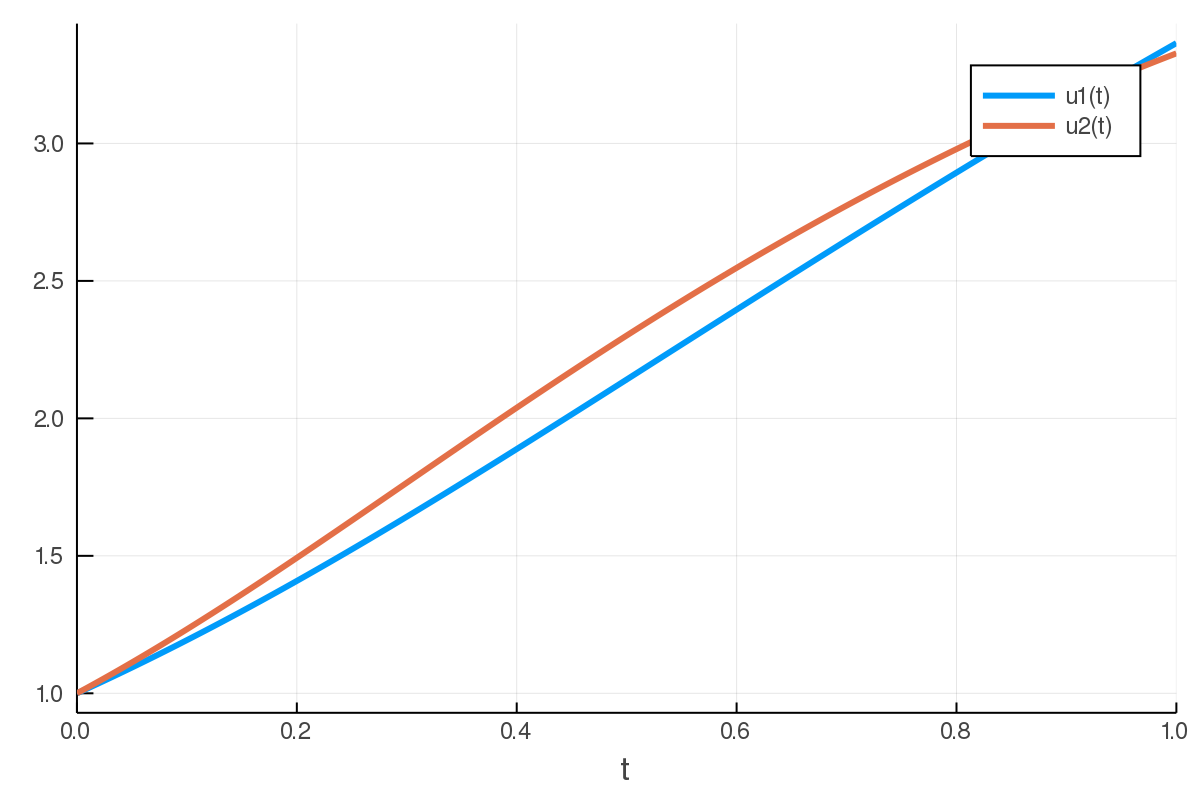
\includegraphics[width=.9\linewidth]{plots/basic.png}
\end{center}

Now, let's use ForwardDiff to verify our results:

\begin{minted}[frame=lines,linenos=true,mathescape,breaklines=true]{julia}
function full(x)
    u0, p = unpack(x, 2, param_count)
    ps = unpack(p, (size(w) for w in ps0)...)
    sol = evaluate(ts, u0, ps)
    fake_loss(sol(t1))
end

correct = ForwardDiff.gradient(full, pack(u0, ps0...))
u̅0_c, p̅0_c = unpack(correct, 2, param_count)

u̅s = [fake_loss_pullback(1.0) for t in ts]
u̅0, p̅s0 = sensitivities(ts, u̅s, u0, ps0)
p̅0 = pack(p̅s0...)

@assert allclose(u̅0_c, u̅0)
@assert allclose(p̅0_c, p̅0)
\end{minted}

It works!!

\section{Problem 4}
\label{sec:org2d884b3}
\begin{minted}[frame=lines,linenos=true,mathescape,breaklines=true]{julia}
loss(us_c_, us_) = sum((us_c_ - us_).^2)
loss_pullback(l̅, us_c, us) = l̅ * -2.0 .* (us_c - us)

u0 = [2.0, 0.0]
ps0 = [W1, W2, b1, b2]
t0 = 0.0
t1 = 1.0
ts = t0:0.1:t1

A = [-0.1 2.0; -2.0 -0.1]

target_problem = ODEProblem((u, p, t) -> A * u, u0, (t0, t1))
target_sol = solve(target_problem, Tsit5(), saveat=ts)
us_c = target_sol.(ts)
us_c_ = hcat(us_c...)'

ps = deepcopy(ps0)

function train(ps; steps=500, α=.0001, snapshot_every=5,
               slow_every=200)
    losses = Float64[]
    snapshots = Any[]

    for i in 1:steps
        if (i-1) % snapshot_every == 0
            push!(snapshots, deepcopy(ps))
        end
        if i % slow_every == 0
            α *= .5
        end

        # we do the forward pass twice here to avoid interpolating between points
        # when computing the gradient
        nn_sol = evaluate(ts, u0, ps)
        us = nn_sol.(ts)
        us_ = hcat(us...)'

        l = loss(us_c_, us_)
        push!(losses, l)

        l̅ = 1.0
        u̅s = loss_pullback(l̅, us_c, us)

        _, p̅s = sensitivities(ts, u̅s, u0, ps)

        ps -= α * p̅s

    end

    ps, losses, snapshots
end

ps, losses, snapshots = train(ps)
nn_sol = evaluate(ts, u0, ps)
png(plot(losses, dpi=200, xlabel="iteration", ylabel="loss"), "plots/loss.png")
\end{minted}

\begin{center}
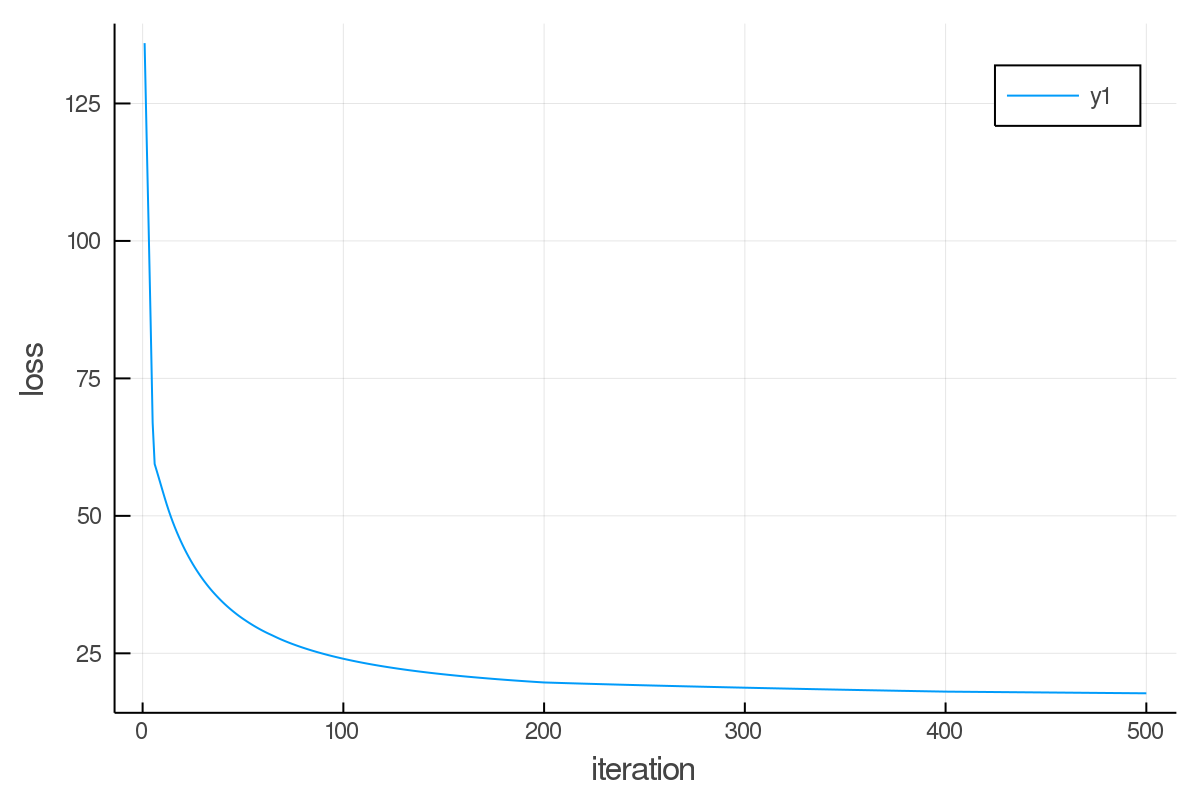
\includegraphics[width=.9\linewidth]{./plots/loss.png}
\end{center}

\begin{minted}[frame=lines,linenos=true,mathescape,breaklines=true]{julia}
p = plot(nn_sol, format=:png, dpi=200, legend=false)
plot!(p, target_sol)

us = nn_sol.(ts)
l̅ = 1.0
u̅s = loss_pullback(l̅, us_c, us)

for i in 1:length(ts)
    t = ts[i]
    plot!(p, Shape([(t, us[i][1]), (t, us[i][1] - .1 * u̅s[i][1])]))
    plot!(p, Shape([(t, us[i][2]), (t, us[i][2] - .1 * u̅s[i][2])]))
end

png(p, "plots/fit.png")
\end{minted}

\begin{center}
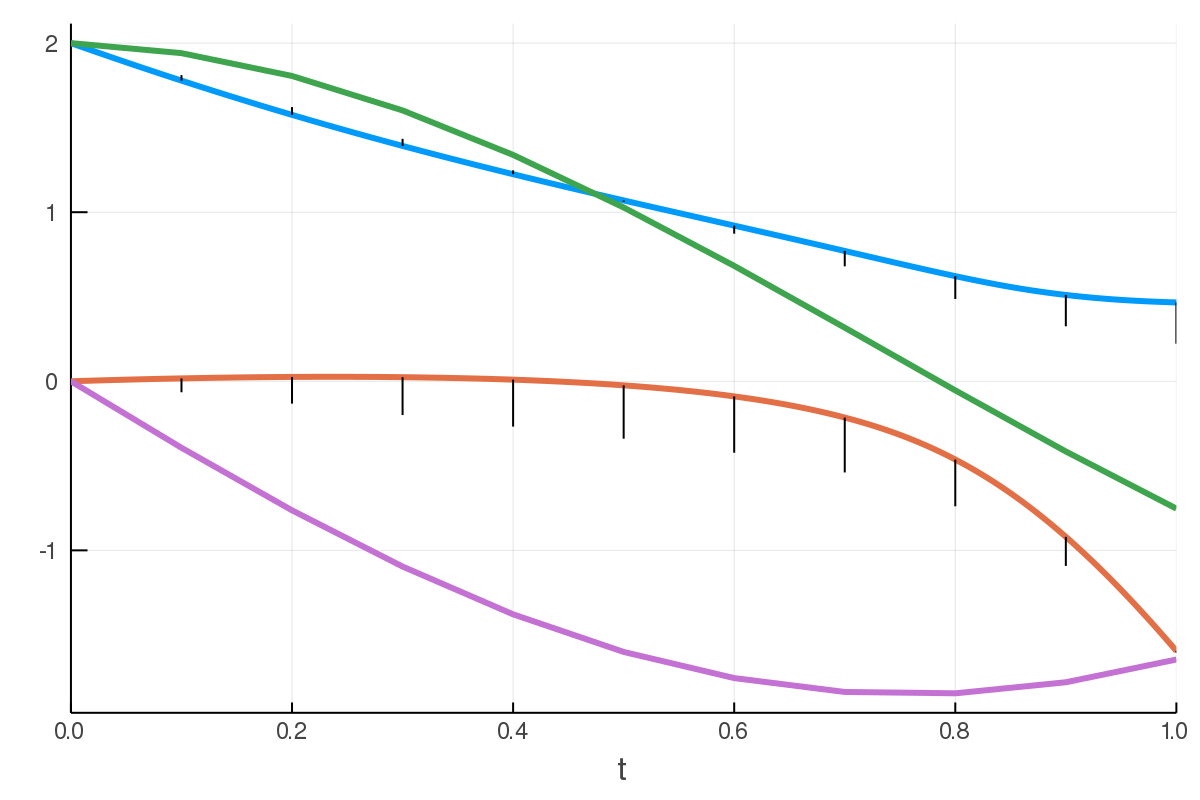
\includegraphics[width=.9\linewidth]{./plots/fit.png}
\end{center}

\begin{minted}[frame=lines,linenos=true,mathescape,breaklines=true]{julia}
function timeplot(snapshots, ts, u0, us_c)
    @gif for ps_ in snapshots
        nn_sol = evaluate(ts, u0, ps_)
        p = plot(nn_sol, ylim=(-2.2, 2.2), legend=false)
        plot!(p, target_sol)

        us = nn_sol.(ts)
        l̅ = 1.0
        u̅s = loss_pullback(l̅, us_c, us)

        for i in 1:length(ts)
            t = ts[i]
            plot!(p, Shape([(t, us[i][1]), (t, us[i][1] - .1 * u̅s[i][1])]))
            plot!(p, Shape([(t, us[i][2]), (t, us[i][2] - .1 * u̅s[i][2])]))
        end

        p
    end
end
timeplot(snapshots, ts, u0, us_c)
\end{minted}
\end{document}
